
\subsection{VM-Centric Snapshot Deletion with Periodic Leak Repair}
\label{sect:delete}


\begin{figure}[htbp]
%\vspace{2em}
  \centering
  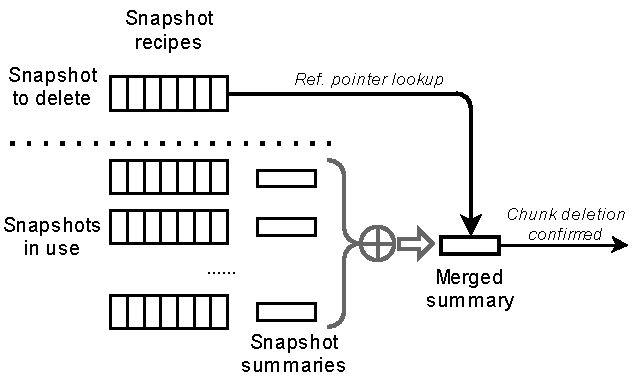
\epsfig{file=images/deletion.pdf, width=3.35in}
  \caption{Fast approximate deletion}
  \label{fig:deletion_flow}
\end{figure}

Snapshot deletions can occur frequently since old snapshots become less useful.
Both space accounting and reclaimation are difficult because deduplication
greatly complicates how we identify unused data when deletion occurs.
To filter out un-referenced data from shared duplicates,
it would require to either maintain expensive live schemas and operations
such as global reference counting,
or use some advanced mark-and-sweep methodologies~\cite{Guo2011,Fabiano2013},
which are all unsuitable for converged architecture as discussed in section~\ref{sect:background}.
% to identify if a chunk can be safely removed without any reference.
%Since our VM-centric design restricts sharing of data chunks only to a small dataset,
%we can greatly simplify the deletion process by 
%focusing on  unreferenced non-PDS chunks within each VM. 
%This process can be conducted independently per VM, and thus results in  a simpler flow control and 
%lower resource usage. 
One of the key benefits of our VM-centric design is that it allows for faster and simpler deletion. 
We propose the following strategies to speedup the deletion process and reduce its resource usage.
\begin{itemize}
\item First, since
sharing in our approach is limited to only a small dataset, we can greatly simplify deletion by focusing
on intra-VM sharing rather than inter-VM sharing. Then the snapshot
 deletion can therefore be conducted independently among VMs.
\item Second,  we propose an {\em approximate} deletion strategy to trade deletion accuracy for speed and
resource usage. Since the VM size is highly skewed in practice,  a large VM may still require
a substantial amount of memory  to facilitate the mark-sweep process of data chunks used within all snapshots
of this VM. 
Our approximate deletion method sacrifices a small percent of storage leakage
to efficiently identify unused chunks using a per-snapshot bloom-filter.
\end{itemize}
The simplified deletion algorithm contains three aspects.
\begin{itemize}
\item {\bf Computation for snapshot reference summary.}
Every time there is a new snapshot created,
we compute a Bloom-filter with $z$ bits as the reference summary vector for all non-PDS chunks used 
in this snapshot.
The items we put into the summary vector are all the references appearing in the metadata of the snapshot.
For each VM we preset the vector size according to estimated VM image size;
given $h$ snapshots stored for a VM, there are $h$ summary vectors maintained.
We adjust the summary vector size and recompute the vectors if the VM size changes substantially over time.
This can be done during periodic leakage repair described below.

\item {\bf Fast approximate deletion with summary comparison.}
When there is a snapshot deletion,  
we identify if chunks to be deleted from that snapshot
are still referenced by other snapshots. 
This is done approximately and quickly by comparing the 
reference of deleted chunks  with
the merged reference summary vectors of other live snapshots.
The merging of live snapshot Bloom-filter vectors uses the bit-wise OR operator 
and the merged vector still takes $z$ bits.
Since the number of live snapshots $h$ is limited for
each VM, 
the time and memory cost of this comparison is small, linear to the number of chunks to be deleted.
If a chunk's reference is not found in the merged summary vector, 
this chunk is not used by any live snapshots. Thus it can be deleted safely.
However, among all the chunks to be deleted, 
there are a small percentage of unused chunks  which
are misjudged as  being in use, resulting in storage leakage.

One advantage of the above fast method is that it can finish  and free storage 
usage immediately, while other offline methods (e.g. ~\cite{Guo2011,Fabiano2013})
can't. That is important for storage accounting as users pay for used storage and delayed deletion
affects the accounting.

\item {\bf Periodic repair of leakage}.
%[exlpain why second Bloom filter, why scan append store]
Leakage repair is conducted periodically to fix the above approximation error.
This procedure compares the live chunks for each VM with what are truly used in the VM snapshot recipes.
A mark-and-sweep process  requires a scan of all the metadata for a snapshot store.
%Our VM-centric mark-and-sweep procedure is similar to Guo\cite{Guo2011} 
%in a way that the data dependency is clearly known.
%This generally requires a scan of almost the entire snapshot store which is much more expensive than approximate deletion,
%although certain optimized algorithms may apply\cite{Przemyslaw2013}. But 
Since it is a VM-specific procedure, 
the space cost is proportional to the number of chunks
within each VM. 
%For example, the space requirement is about 85MB for a VM of size 40GB in our tested dataset.
 This is  much less expensive  than  the VM-oblivious mark-and-sweep
which scans snapshot chunks from all VMs, even with optimization~\cite{Guo2011}.

%Given $n$ VMs in a cluster, the space cost is $n$ times larger.
%For example, consider each reference consumes 8 bytes plus  1 mark bit. A VM that has 40GB backup data with about
%10 million chunks will need less than 85MB of memory to complete a VM-specific mark-and-sweep process
%in less than half an hour, assuming 50MB/s disk bandwidth is allocated.
\end{itemize}

%{\bf Discussion}
We estimate storage leakage size and how often leak repair should be conducted.
Assume that  a VM keeps $h$ snapshots in backup storage, creates and deletes one snapshot
every day. Let $u$ be the number of chunks brought by initial backup for a VM, $\Delta u$ be the average
number of additional chunks added from one version to next snapshot version. Then the total number of 
chunks in a VM's snapshot store is about:
$
U = u + (h-1)\Delta u.
$

Each Bloom filter vector has  $z$ bits for each snapshot and let $j$ be the number of hash functions used by the
Bloom filter.  Notice that a chunk may appear multiple times in these summary vectors; however, this should not 
increase the probability of being a 0 bit in all $h$ summary vectors.
Thus the probability that a particular bit is 0  in all $h$ summary vectors is  
\[
(1- \frac{1}{z}) ^{j U}.
\] 
Then the misjudgment rate of being in use  is: 
\begin{equation}
\label{eq:falserate}
\epsilon = (1-(1-\frac{1}{z})^{jU})^j.
\end{equation}

For each snapshot deletion, the number of chunks to be deleted is nearly identical to the number of
newly added chunks $\Delta u$. 
Let $R$ be the total number of runs of approximate deletion between two consecutive 
repairs. We estimate  the total leakage $L$ after $R$ runs as:
\[
L = R \epsilon \Delta u.
\]
When leakage ratio $L/U$ exceeds a pre-defined threshold $\tau$, we trigger a leak repair. Namely,

\begin{equation}
\label{eq:leakrepair}
\frac{L}{U} = \frac{R \Delta u \epsilon}{u+(h-1)\Delta u } > \tau 
\Longrightarrow R > \frac{\tau}{\epsilon}\times\frac{u + (h-1)\Delta u}{\Delta u}.
\end{equation}

For example for our test data in Section~\ref{sect:evaluation},  
$h=10$ and each snapshot adds
about 0.1-5\% of new data. Thus ${\Delta u}/{u} \approx 0.025$. For a 40GB snapshot, $u\approx  10$ million.
Then $U=12.25$ million.
We choose  $\epsilon = 0.01$ and $\tau=0.05$.  From Equation~\ref{eq:falserate}, 
each summary vector requires $z=10U=122.5$ million bits or 15MB. From Equation~\ref{eq:leakrepair}, 
leak repair should be triggered once for every R=245 runs of approximate deletion. 
When one machine hosts 25 VMs and there is one snapshot deletion per day per VM, there would be 
only one full leak repair for one physical machine scheduled for every 9.8 days. 
If $\tau = 0.1$ then leakage repair would occur every 19.6 days.

